\section{Summary}

\begin{itemize}
\item SPDHG excellent alg for non-smooth priors, but only sinogram
\item modern TOF PET data is extremly sparse (Figure) -> SPDHG inefficient
      in terms of memory and speed
\item LM projections are much faster than sino projections for usual count levels
      (Table)
\item propose LM-SPDHG that solves both issues
\item 1st step: better init
\item 2nd step: rewrite SPDHG in terms of LM updates
\end{itemize}

\section{Materials and Methods}

\subsection{Problem}

\begin{equation}
\argmin _{x\geq 0} \sum_{i=1}^{n} \underbrace{(Px + s)_i -  d_i \log \left( (Px + s)_i \right)}_{D_i(x)} + R (K x),
\end{equation}

\begin{equation}
\argmin _{x\geq 0} \, \sup_{y,w} \,  \langle Px + s, y \rangle + \langle Kx, w \rangle - \sum_{i=1}^{n} D_i^*(y_i) - R^*(w),
\end{equation}

\begin{equation}
D_i^*(y_i) =
\begin{cases}
-d_i + d_i \log \left( \frac{d_i}{1-y_i} \right) & \text{if } y_i \leq 1 \\
\infty & \text{else}
\end{cases}
\end{equation}

\begin{equation}
(\prox_{D_i^*}^{S}(y))_i = \frac{1}{2} \left(y_i + 1 - \sqrt{ (y_i-1)^2 + 4 S_i d_i} \right)
\label{eq:proxD}
\end{equation} 

\subsection{Better intialization of sinogram SPDHG}

Use quick EM-TV (e.g. 1 iteration 28 susbets) as initializtion for $x$.
Initialize $y$ (dual variable of data) as
\begin{equation}
y^0 = 1 - \frac{d}{Px^0 + s} \ .
\end{equation}
Note that this also means that the initial y is 1 in bins where we have
no data such that we don't need to keep y in memory during the iterations.

(optionally) intialize $w$ (dual of gradient) in subgradient of $R(Kx^0)$

%-----------------------------------------------------------------------------
\begin{algorithm}[t]
\begin{algorithmic}[1]
\small
\State \textbf{Initialize} $x(=0),y(=0),(w=0)$, $(S_i)_i,T,(p_i)_i$,
\State $\overline{z} = z = P^T y + K^T w$
\Repeat
	\State $x = \proj_{\geq 0} (x - T \overline{z})$
	\State Select $i \in \{ 1,\ldots,n+1\} $ randomly according to $(p_i)_i$
  \If{$i \leq n$}
	\State $y_i^+ \gets \prox_{D_i^*}^{S_i} ( y_i + S_i  ( P_i x + s_i))$
	\State $\delta z \gets P_i^T (y_i^+ - y_i)$
	\State $y_i \gets y_i^+$
  \Else
	\State $w^+ \gets \prox_{R^*}^{S_i} ( w + S_i  K x)$
	\State $\delta z \gets K^T (w^+ - w)$
	\State $w \gets w^+$
  \EndIf
	\State $z \gets z + \delta z$
	\State $\overline{z} \gets  z + (\delta z/p_i)$
\Until{stopping criterion fulfilled}
\State \Return{$x$}
%\EndFunction
\end{algorithmic}
\caption{SPDHG for PET reconstruction}
\label{alg:spdhg}
\end{algorithm}




%-----------------------------------------------------------------------------
\begin{algorithm}[t]
\begin{algorithmic}[1]
\small
\State \textbf{Input} event list $N$
\State \textbf{Calculate} event counts $\mu_e$ for each e in $N$ (see text)
\State \textbf{Split} event list $N$ into $m$ sublists $N_i$
\State \textbf{Initialize} $x,w,(S_i)_i,T,(p_i)_i$
\State \textbf{Preprocessing} $\overline{z} = z = P^T y + K^T w$ (see text)
\State \textbf{Initialize} $m$ sub lists $l_{N_i}$ with 0s
\Repeat
	\State $x = \proj_{\geq 0} (x - T \overline{z})$
	\State Select $i \in \{1,\ldots,m+1\}$ randomly accord. to $(p_i)_i$
  \If{$i \leq m$}
	  \State $l_{N_i}^+ \gets \prox_{D^*}^{S_i} \left( l_{N_i} + S_i \left(P^{LM}_{N_i} x + s_{N_i} \right) \right)$
	  \State $\delta z \gets {P^{LM}_{N_i}}^T \left(\frac{l_{N_i}^+ - l_{N_i}}{\mu_{N_i}}\right)$
	  \State $l_{N_i} \gets l_{N_i}^+$
  \Else
	  \State $w^+ \gets \prox_{R^*}^{S_i} \left( w + S_i K x \right)$
	  \State $\delta z \gets K^T \left(w^+ - w\right)$
	  \State $w \gets w^+$
  \EndIf
	\State $z \gets z + \delta z$
	\State $\overline{z} \gets  z + (\delta z/p_i)$
\Until{stopping criterion fulfilled}
\State \Return{$x$}
%\EndFunction
\end{algorithmic}
\caption{LM-SPDHG for PET reconstruction}
\label{alg:lmspdhg}
\end{algorithm}


%-----------------------------------------------------------------------------

\section{Results}

\begin{figure*}
  \centering
    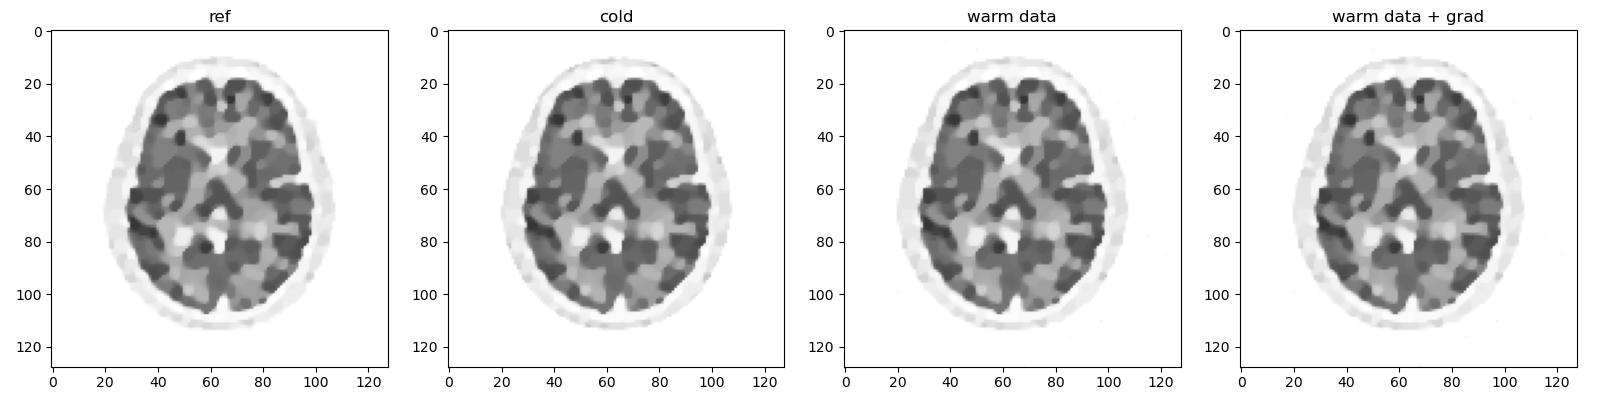
\includegraphics[width=1.0\textwidth]{figs/SPDHG_sino_init.png}
    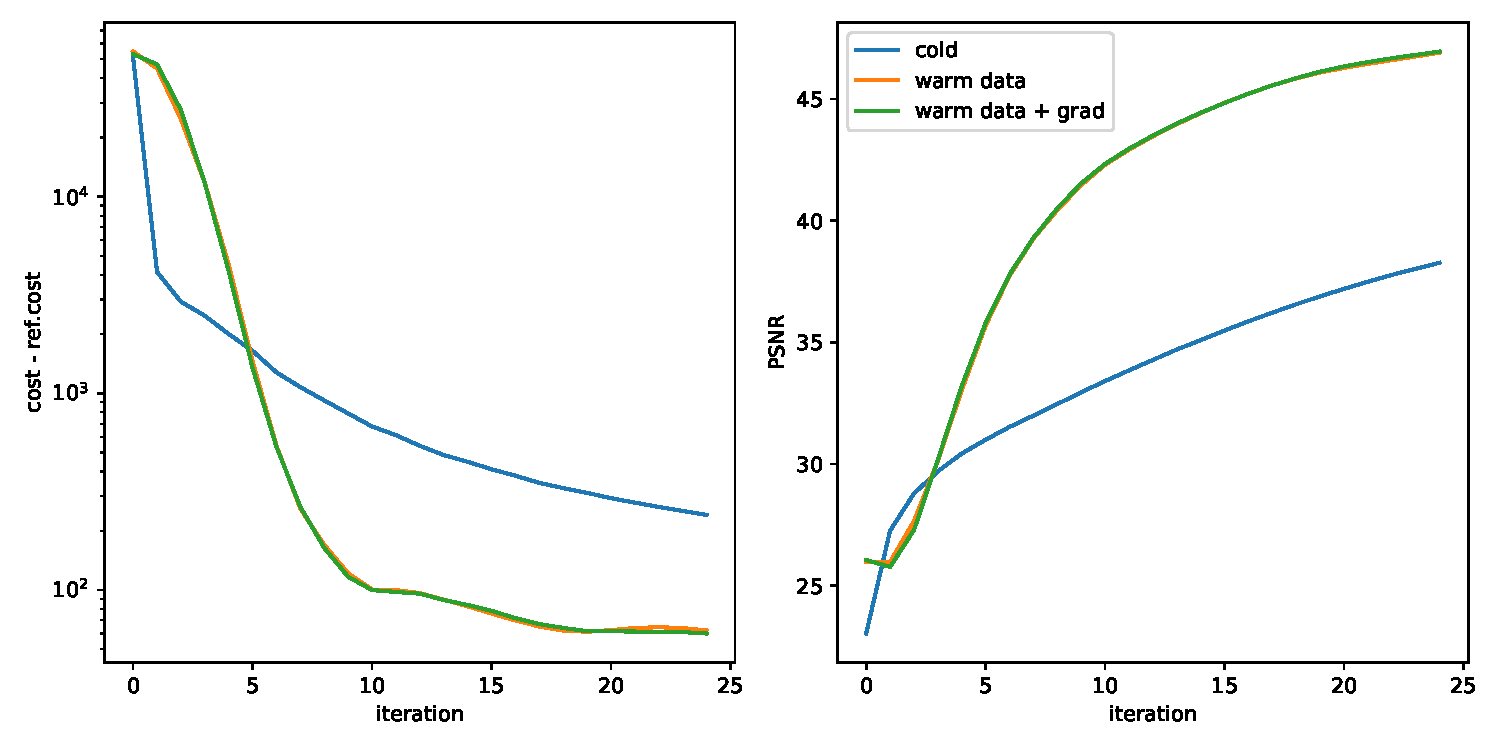
\includegraphics[width=0.8\textwidth]{figs/SPDHG_sino_init_metrics.pdf}
  \caption{$1\cdot10^6$ counts, DTV, $\beta = 0.03$, 112 subsets sinogram SPDHG. ``warm'' start leads to faster convergence in the early iterations.}
  \label{fig:metrics}
\end{figure*}


\begin{figure*}
  \centering
    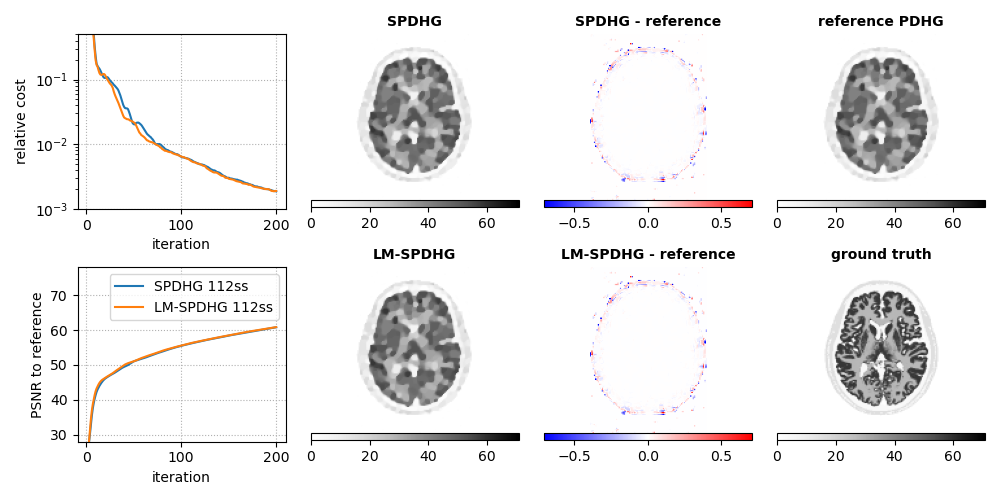
\includegraphics[width=1.0\textwidth]{./figs/brain2d_counts_1.0E+06_seed_1_beta_3.0E-02_prior_TV_niter_ref_20000_fwhm_4.5_4.5_niter_200.png}
    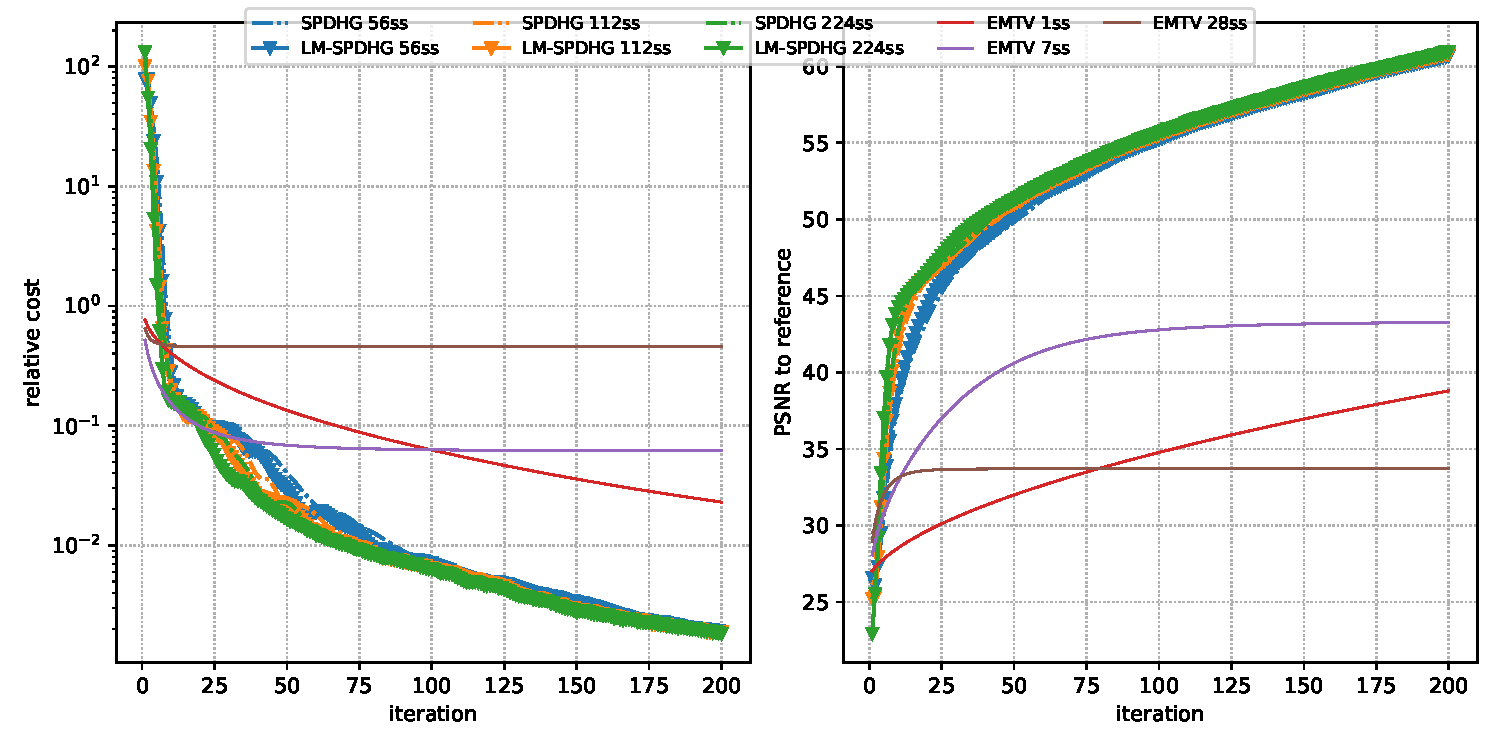
\includegraphics[width=0.8\textwidth]{./figs/brain2d_counts_1.0E+06_seed_1_beta_3.0E-02_prior_TV_niter_ref_20000_fwhm_4.5_4.5_niter_200_metrics.pdf}
  \caption{$1\cdot10^6$ counts, TV, $\beta = 0.03$}
  \label{fig:metrics}
\end{figure*}

\begin{figure*}
  \centering
    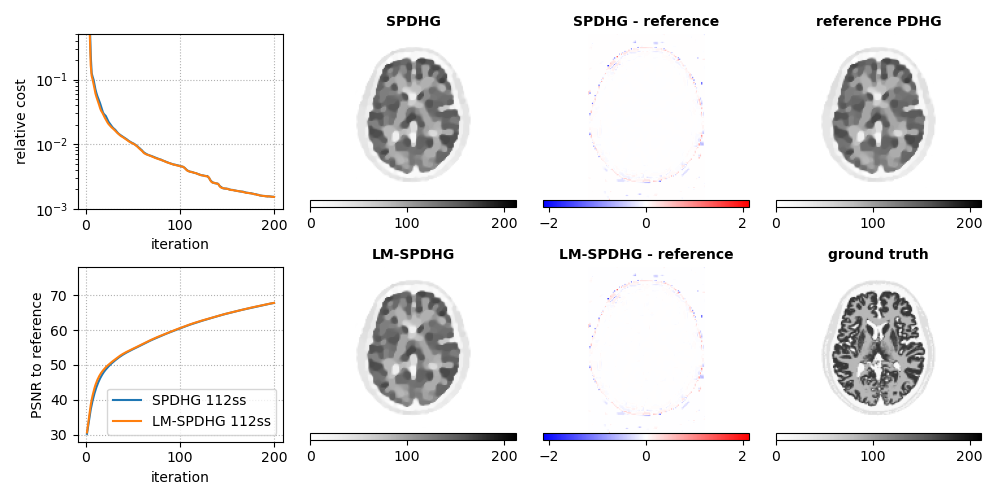
\includegraphics[width=1.0\textwidth]{./figs/brain2d_counts_3.0E+06_seed_1_beta_3.0E-02_prior_TV_niter_ref_20000_fwhm_4.5_4.5_niter_200.png}
    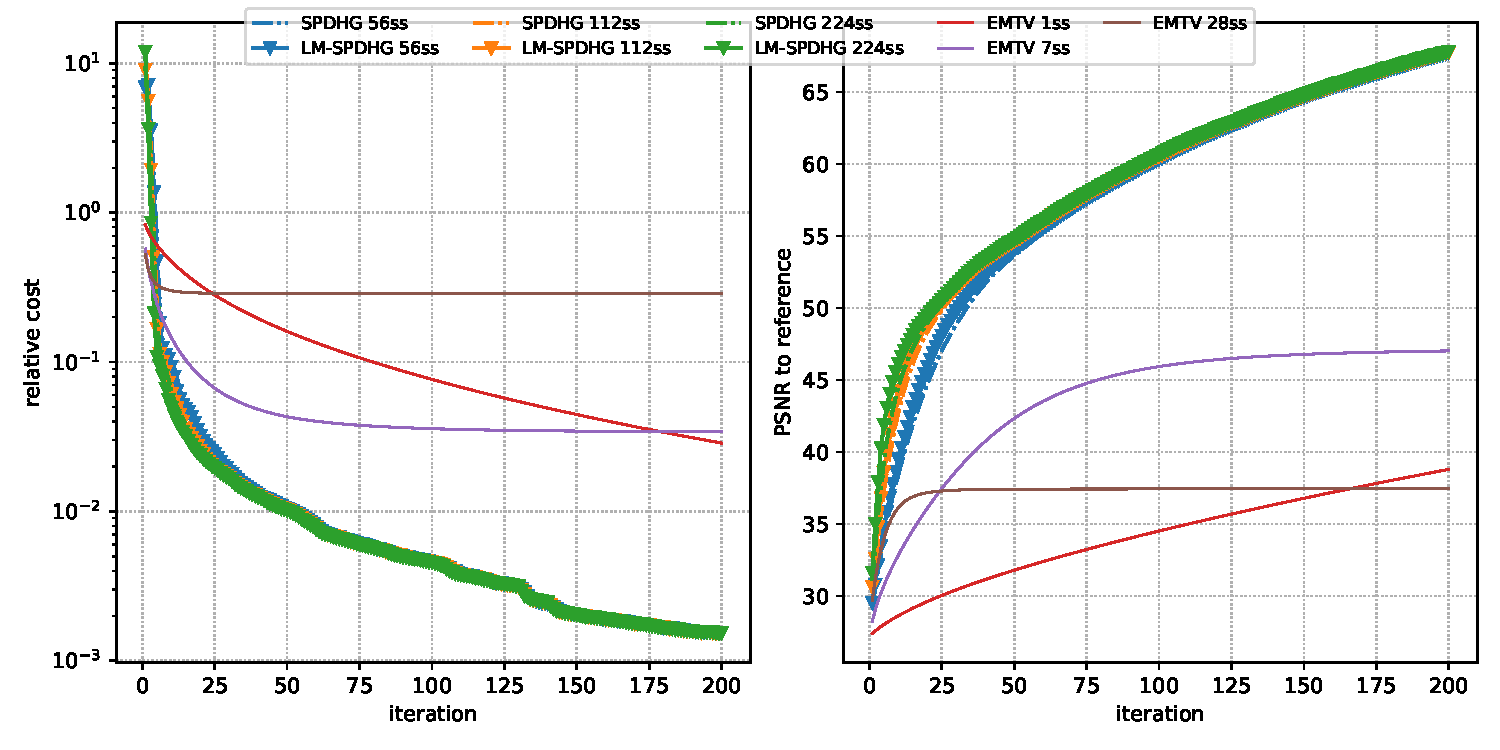
\includegraphics[width=0.8\textwidth]{./figs/brain2d_counts_3.0E+06_seed_1_beta_3.0E-02_prior_TV_niter_ref_20000_fwhm_4.5_4.5_niter_200_metrics.pdf}
  \caption{$3\cdot10^6$ counts, TV, $\beta = 0.03$}
  \label{fig:metrics}
\end{figure*}

\begin{figure*}
  \centering
    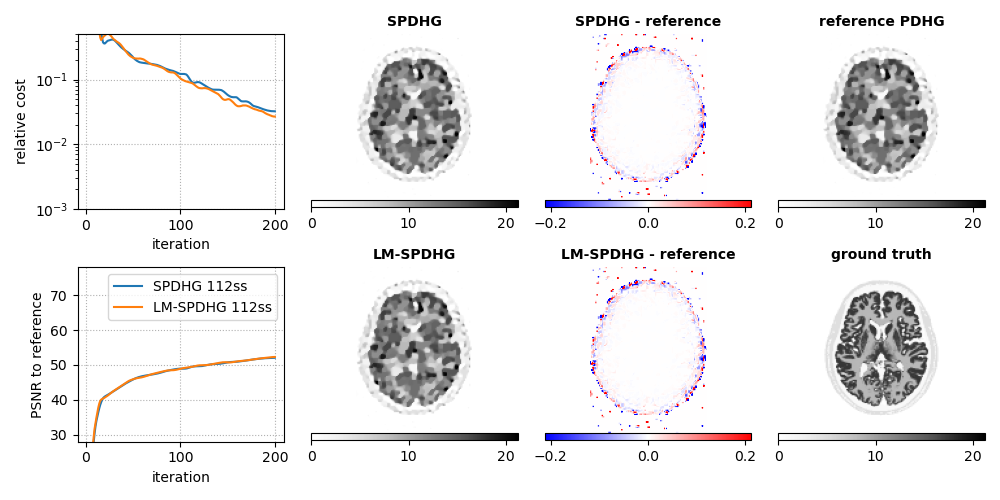
\includegraphics[width=1.0\textwidth]{./figs/brain2d_counts_3.0E+05_seed_1_beta_3.0E-02_prior_TV_niter_ref_20000_fwhm_4.5_4.5_niter_200.png}
    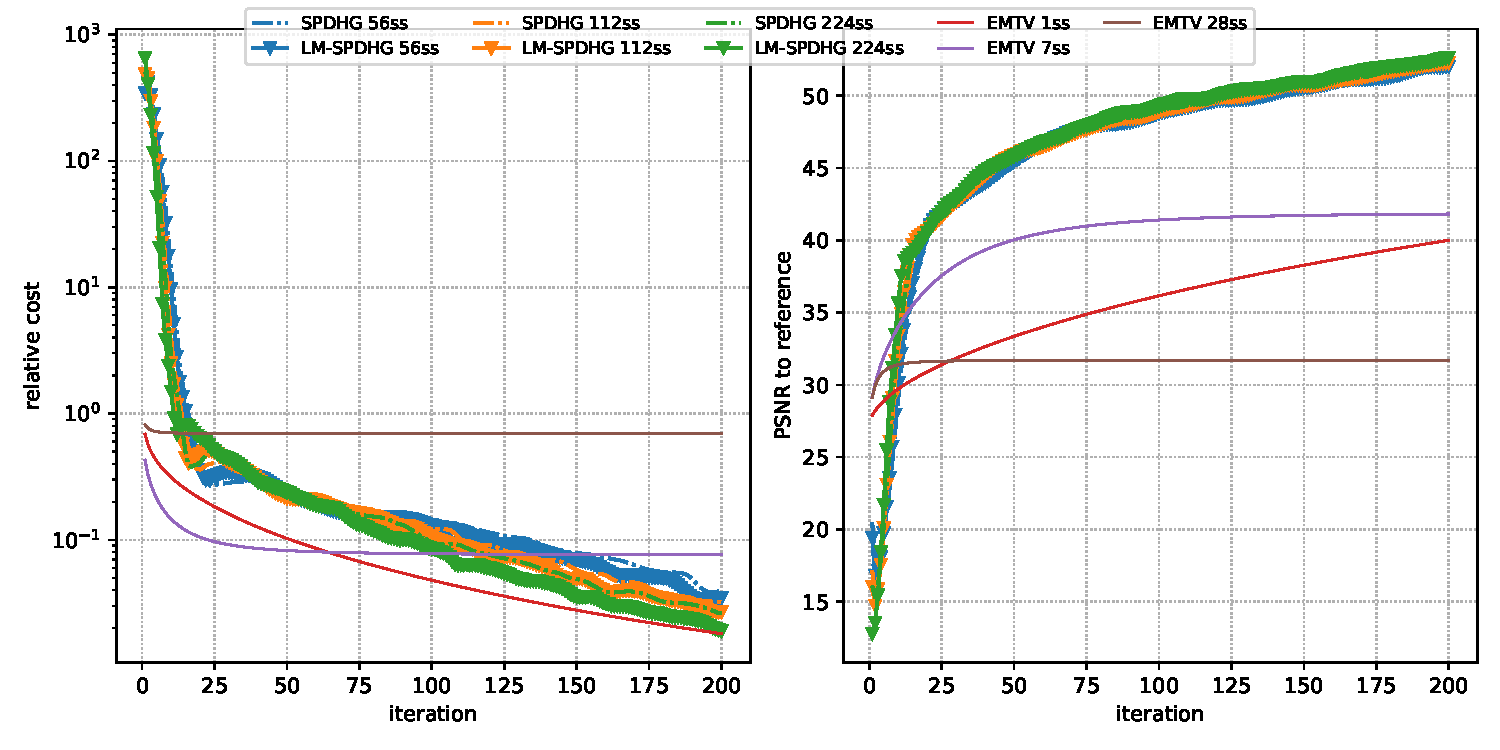
\includegraphics[width=0.8\textwidth]{./figs/brain2d_counts_3.0E+05_seed_1_beta_3.0E-02_prior_TV_niter_ref_20000_fwhm_4.5_4.5_niter_200_metrics.pdf}
  \caption{$3\cdot10^5$ counts, TV, $\beta = 0.03$}
  \label{fig:metrics}
\end{figure*}

\begin{figure*}
  \centering
    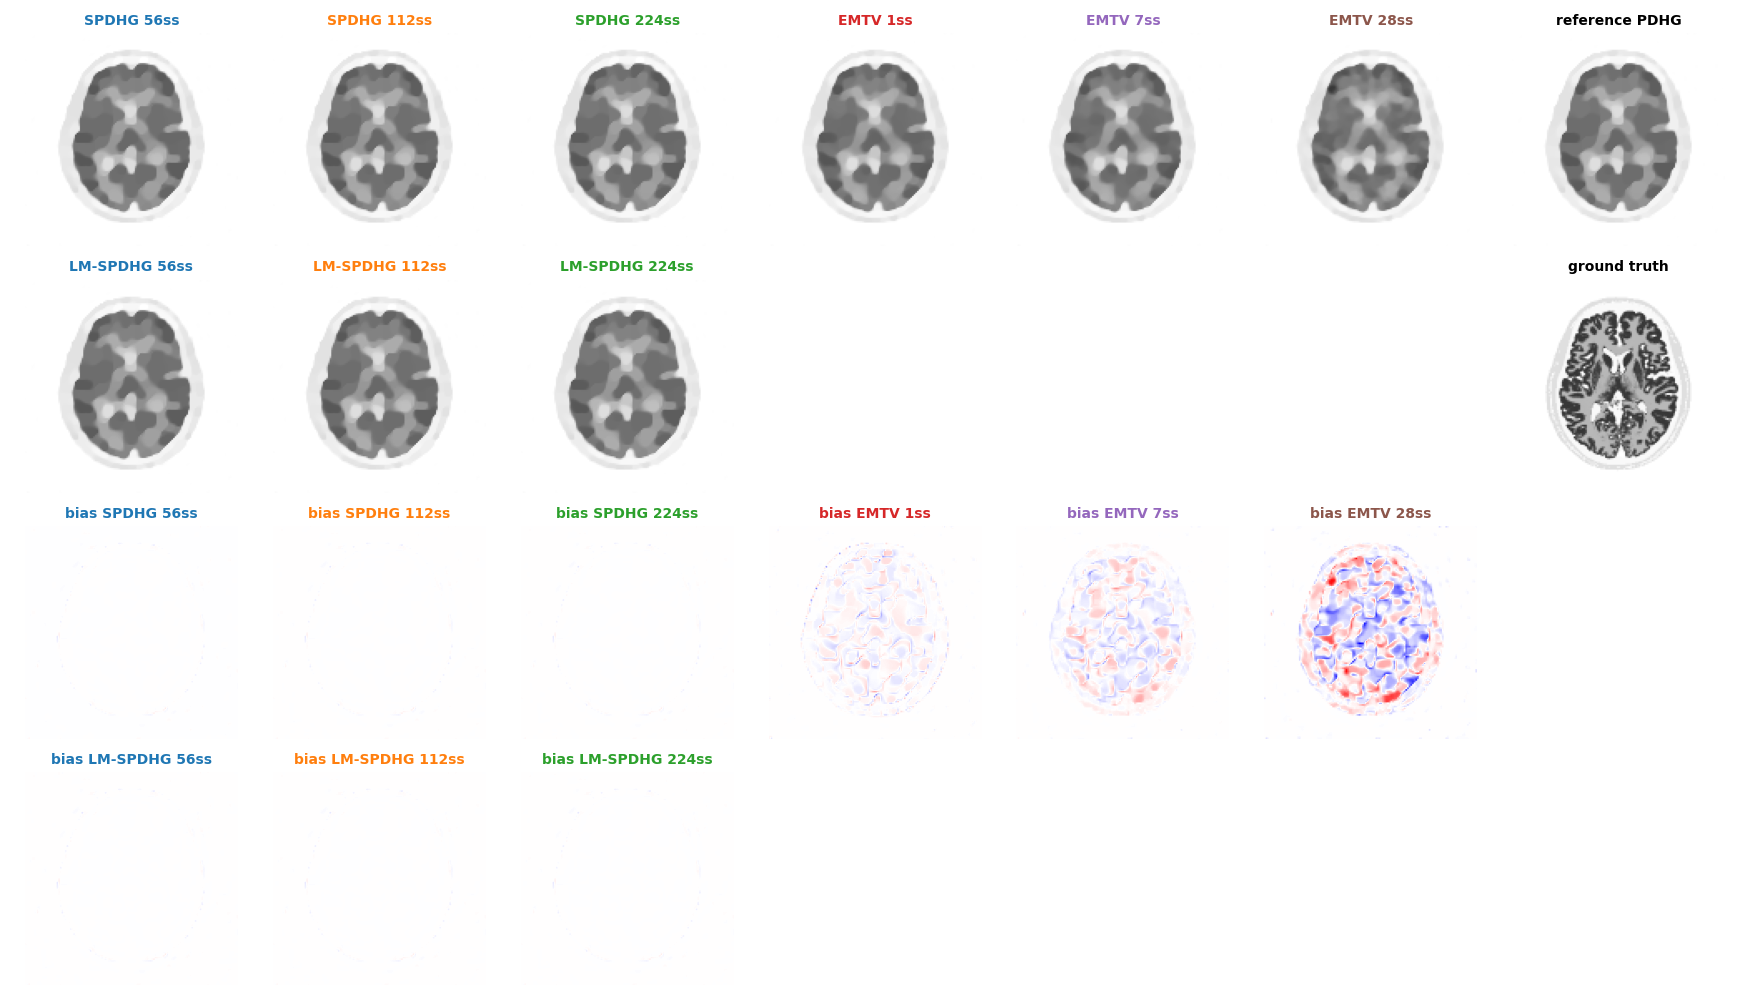
\includegraphics[width=1.0\textwidth]{./figs/brain2d_counts_1.0E+06_seed_1_beta_1.0E-01_prior_TV_niter_ref_20000_fwhm_4.5_4.5_niter_200.png}
    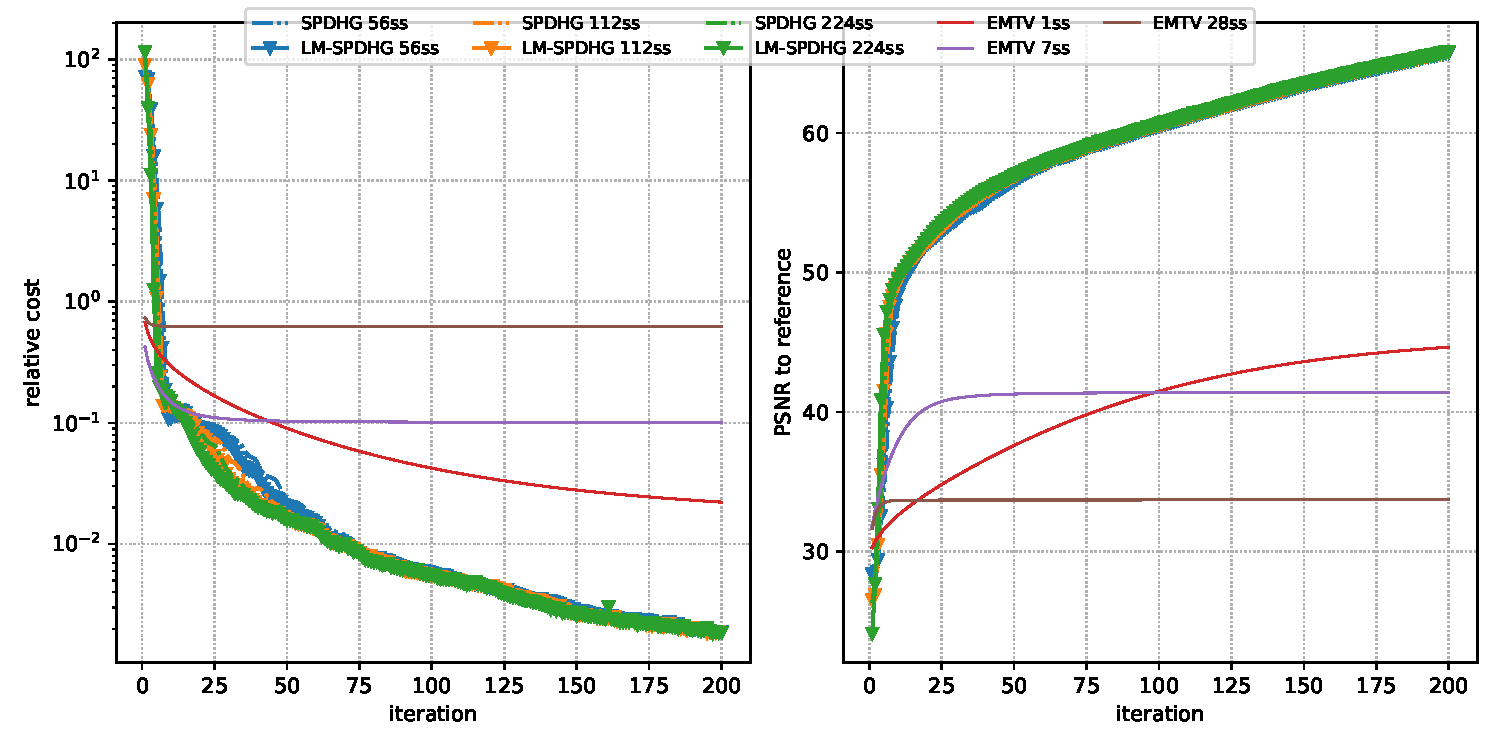
\includegraphics[width=0.8\textwidth]{./figs/brain2d_counts_1.0E+06_seed_1_beta_1.0E-01_prior_TV_niter_ref_20000_fwhm_4.5_4.5_niter_200_metrics.pdf}
  \caption{$1\cdot10^6$ counts, TV, $\beta = 0.1$}
  \label{fig:metrics}
\end{figure*}

\begin{figure*}
  \centering
    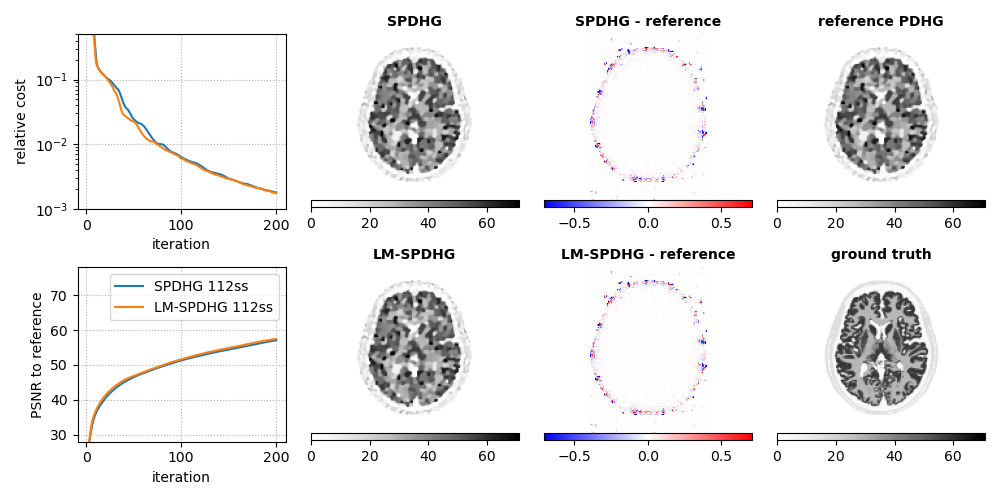
\includegraphics[width=1.0\textwidth]{./figs/brain2d_counts_1.0E+06_seed_1_beta_1.0E-02_prior_TV_niter_ref_20000_fwhm_4.5_4.5_niter_200.png}
    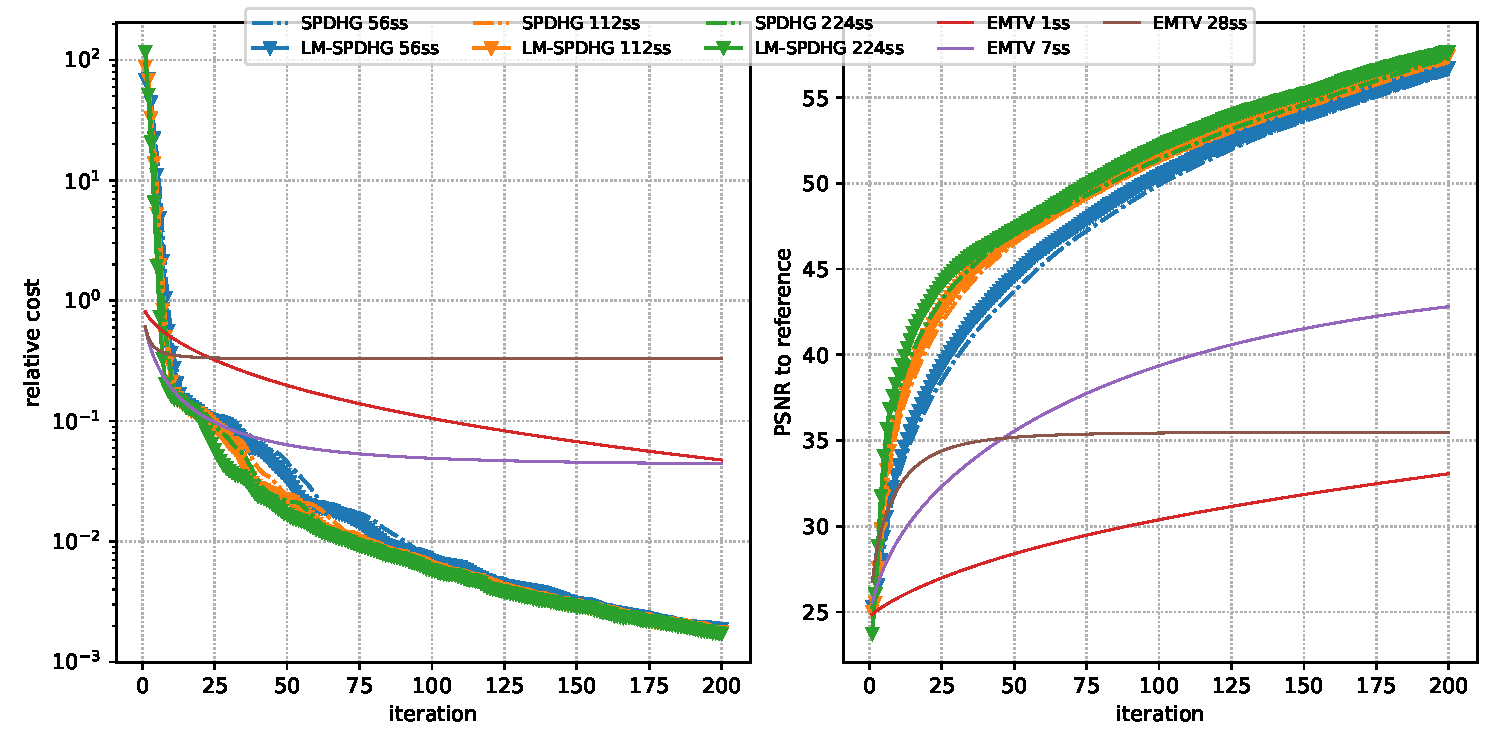
\includegraphics[width=0.8\textwidth]{./figs/brain2d_counts_1.0E+06_seed_1_beta_1.0E-02_prior_TV_niter_ref_20000_fwhm_4.5_4.5_niter_200_metrics.pdf}
  \caption{$1\cdot10^6$ counts, TV, $\beta = 0.01$}
  \label{fig:metrics}
\end{figure*}

\begin{figure*}
  \centering
    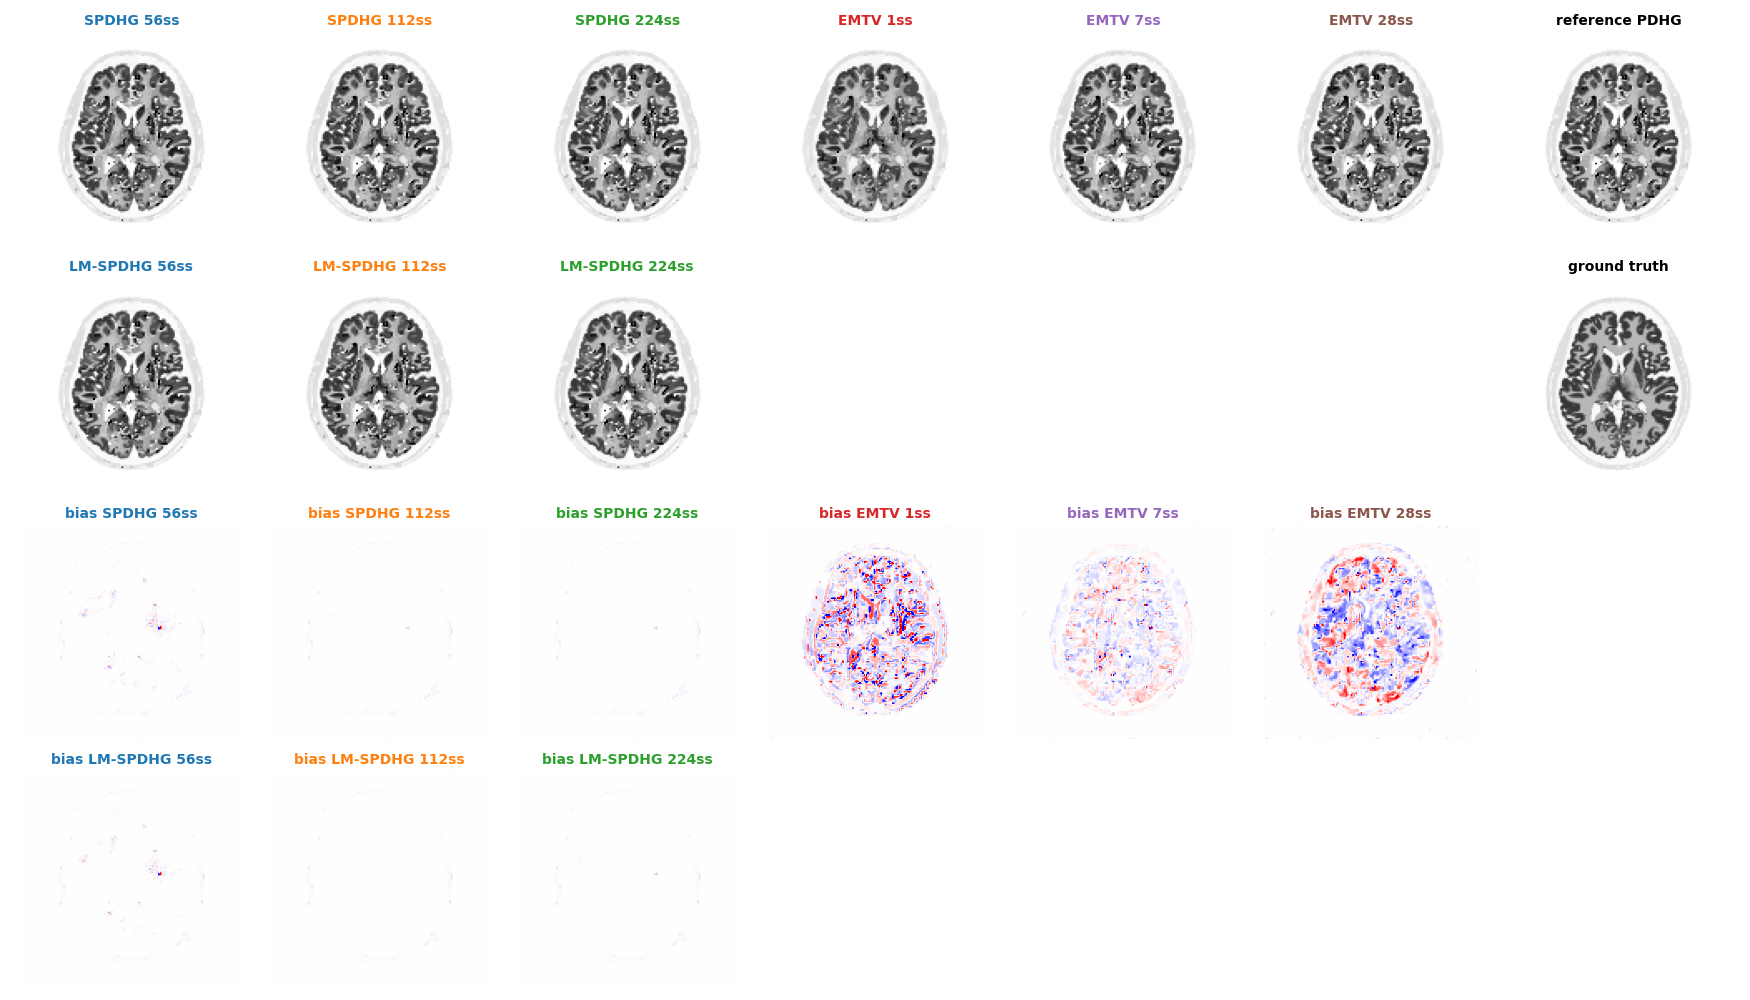
\includegraphics[width=1.0\textwidth]{./figs/brain2d_counts_1.0E+06_seed_1_beta_1.0E-01_prior_DTV_niter_ref_20000_fwhm_4.5_4.5_niter_200.png}
    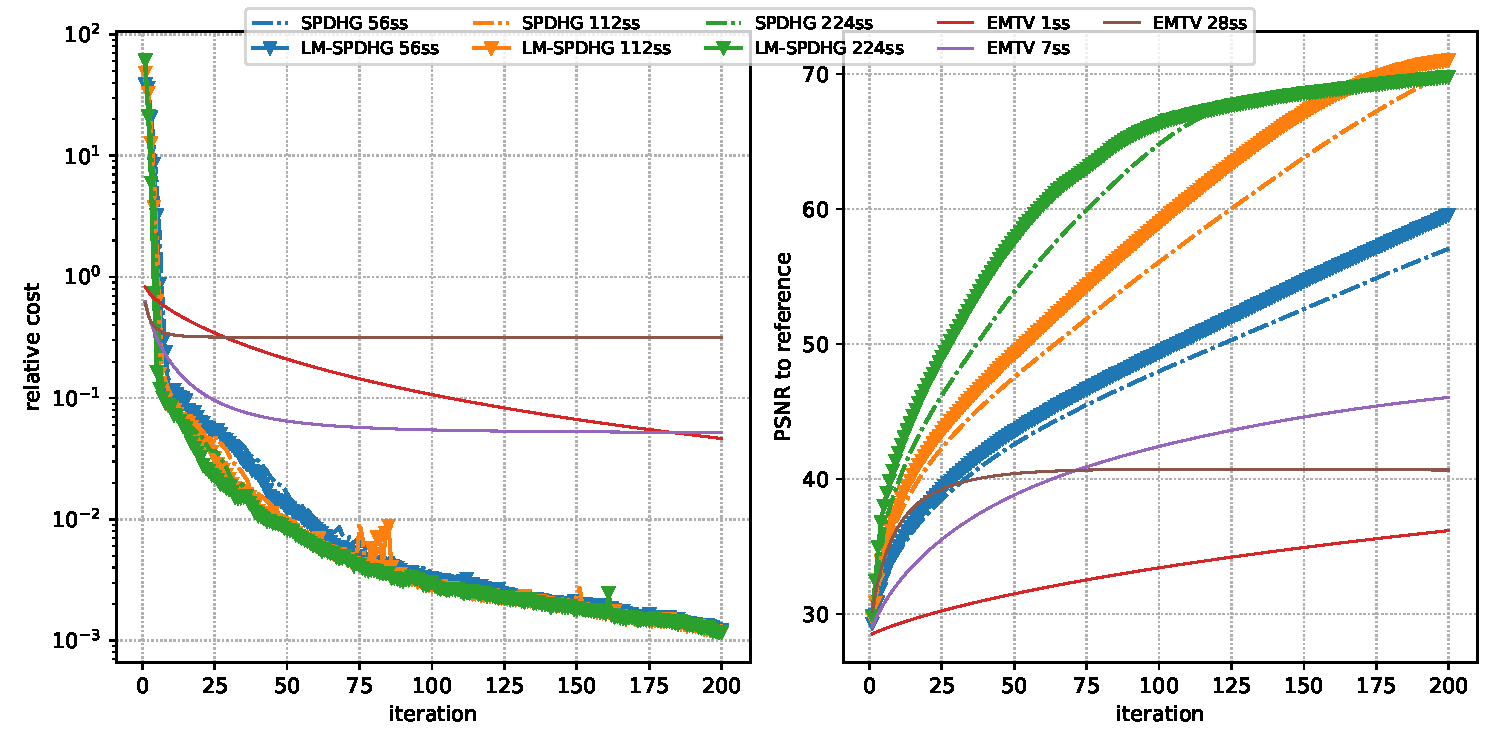
\includegraphics[width=0.8\textwidth]{./figs/brain2d_counts_1.0E+06_seed_1_beta_1.0E-01_prior_DTV_niter_ref_20000_fwhm_4.5_4.5_niter_200_metrics.pdf}
  \caption{$1\cdot10^6$ counts, DTV, $\beta = 0.1$}
  \label{fig:metrics}
\end{figure*}
